\documentclass[tikz,border=0pt]{standalone}
% Shared visual language for every block diagram in figures/diagrams.
% Build with XeLaTeX (see figures/diagrams/build.sh).
\usepackage{fontspec}
\setmainfont{Inter}[Numbers=Lining]
\setmonofont{DejaVu Sans Mono}[Scale=0.86]
\usepackage{xcolor}
\usetikzlibrary{arrows.meta,positioning,calc,fit,backgrounds,shapes.geometric,
  shapes.misc,matrix,decorations.pathreplacing,patterns,quotes}

% Palette (matches python/figstyle.py) --------------------------------------
\definecolor{surface}{HTML}{FCFCFB}
\definecolor{ink}{HTML}{0B0B0B}
\definecolor{ink2}{HTML}{52514E}
\definecolor{muted}{HTML}{898781}
\definecolor{hair}{HTML}{E1E0D9}
\definecolor{memline}{HTML}{2A78D6}  \definecolor{memfill}{HTML}{E7F0FC}
\definecolor{aluline}{HTML}{14875E}  \definecolor{alufill}{HTML}{E3F5EE}
\definecolor{ctlline}{HTML}{B07800}  \definecolor{ctlfill}{HTML}{FDF2D9}
\definecolor{regline}{HTML}{6250D6}  \definecolor{regfill}{HTML}{ECEAFB}
\definecolor{wire}{HTML}{3D3C39}
\definecolor{accent}{HTML}{EB6834}   \definecolor{accentfill}{HTML}{FDE8DF}
\definecolor{pos}{HTML}{E34948}      \definecolor{posfill}{HTML}{FBE1E0}
\definecolor{neg}{HTML}{2A78D6}      \definecolor{negfill}{HTML}{DCE9FA}
\definecolor{zerofill}{HTML}{F0EFEC}

\tikzset{
  every picture/.style={line cap=round, line join=round, font=\small, text=ink},
  % canvas
  canvas/.style={show background rectangle,
    background rectangle/.style={fill=surface, draw=hair, rounded corners=8pt, line width=0.6pt},
    inner frame xsep=16pt, inner frame ysep=14pt},
  ttl/.style={font=\bfseries\large, anchor=north west, inner sep=0pt, text=ink},
  sub/.style={font=\small, anchor=north west, inner sep=0pt, text=ink2},
  % blocks
  blk/.style={rounded corners=3pt, line width=0.8pt, align=center, minimum height=9mm,
    inner xsep=5pt, inner ysep=3pt},
  mem/.style={blk, draw=memline, fill=memfill},
  alu/.style={blk, draw=aluline, fill=alufill},
  ctl/.style={blk, draw=ctlline, fill=ctlfill},
  reg/.style={blk, draw=regline, fill=regfill, rounded corners=1pt},
  io/.style={blk, draw=muted, fill=white},
  ghost/.style={blk, draw=muted, dashed, fill=surface},
  % arithmetic primitives
  add/.style={circle, draw=aluline, fill=white, line width=0.8pt, minimum size=6.2mm,
    inner sep=0pt, font=\normalsize},
  shf/.style={rectangle, rounded corners=1.5pt, draw=aluline, fill=white, line width=0.7pt,
    font=\ttfamily\footnotesize, inner xsep=2.5pt, inner ysep=2pt, minimum height=5mm},
  gain/.style={isosceles triangle, isosceles triangle apex angle=60, draw=aluline, fill=white,
    line width=0.7pt, inner sep=1.2pt, font=\footnotesize},
  dn/.style={circle, draw=wire, fill=white, line width=0.7pt, minimum size=8mm, inner sep=0pt,
    font=\footnotesize},
  mux/.style={trapezium, trapezium angle=72, shape border rotate=270, draw=ctlline, fill=ctlfill,
    line width=0.8pt, minimum height=13mm, minimum width=5mm, inner sep=1pt, font=\scriptsize},
  net/.style={draw=memline, fill=memfill, rounded corners=1.5pt, font=\footnotesize, inner xsep=3pt,
    inner ysep=1.6pt, minimum width=5.5mm, minimum height=4.8mm},
  % wires
  sig/.style={-{Latex[length=2.2mm,width=1.6mm]}, draw=wire, line width=0.75pt},
  bus/.style={-{Latex[length=2.6mm,width=2mm]}, draw=wire, line width=1.5pt},
  ctrl/.style={-{Latex[length=1.8mm,width=1.4mm]}, draw=ctlline, line width=0.65pt, dash pattern=on 3pt off 2pt},
  nohead/.style={-, draw=wire, line width=0.75pt},
  dot/.style={circle, fill=wire, inner sep=0pt, minimum size=3.2pt},
  % labels
  lbl/.style={font=\footnotesize, text=ink2, fill=surface, inner sep=1.2pt},
  lblc/.style={font=\footnotesize, text=ink2, inner sep=1.2pt},
  note/.style={font=\footnotesize, text=ink2, align=left, inner sep=0pt},
  head/.style={font=\bfseries\small, text=ink, inner sep=0pt},
  code/.style={font=\ttfamily\footnotesize, text=ink},
  group/.style={draw=hair, fill=white, rounded corners=6pt, line width=0.8pt, inner sep=7pt},
  grouplabel/.style={font=\bfseries\footnotesize, text=muted, anchor=south west, inner sep=2pt},
}

% Layers: groups sit above the canvas background and below the main layer.
\pgfdeclarelayer{groups}
\pgfsetlayers{background,groups,main}

% A register: box with a clock wedge at the bottom edge.
\newcommand{\clk}[1]{\draw[regline, line width=0.6pt] ($(#1.south)+(-1.4mm,0)$) -- ($(#1.south)+(0,1.6mm)$) -- ($(#1.south)+(1.4mm,0)$);}
% Bus width tick: \bw{(point)}{width}
\newcommand{\bw}[2]{\draw[wire, line width=0.6pt] ($#1+(-0.9mm,-1.2mm)$) -- ($#1+(0.9mm,1.2mm)$); \node[font=\scriptsize, text=ink2, above=0.4mm, inner sep=0.5pt] at #1 {#2};}
\newcommand{\var}[1]{\textit{#1}}
\newcommand{\usub}[1]{\ifcase#1 ₀\or ₁\or ₂\or ₃\or ₄\or ₅\fi}
\AtBeginDocument{\hyphenpenalty=10000\exhyphenpenalty=10000}

\begin{document}
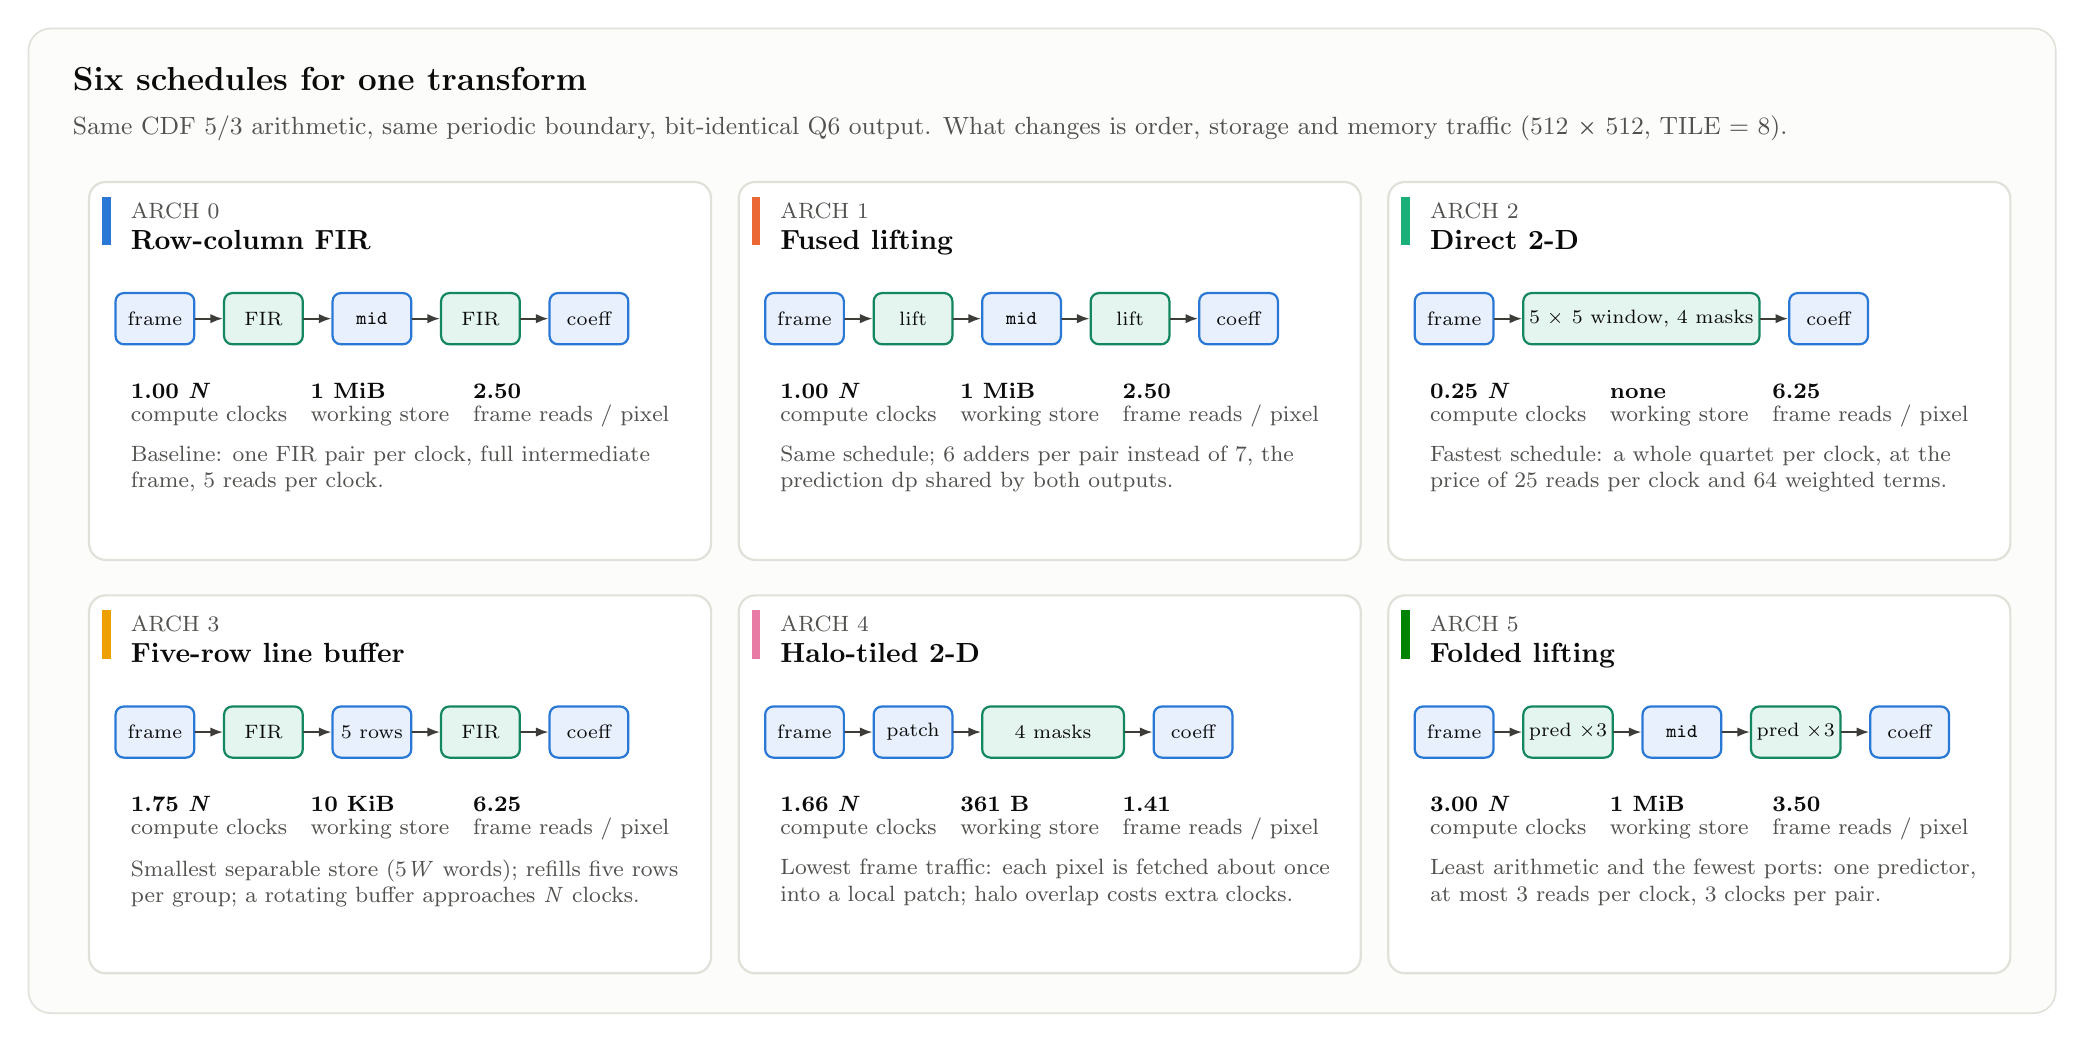
\begin{tikzpicture}[canvas]
  \node[ttl] at (0,0) {Six schedules for one transform};
  \node[sub] at (0,-0.62) {Same CDF 5/3 arithmetic, same periodic boundary, bit-identical Q6 output. What changes is order, storage and memory traffic (512 × 512, TILE = 8).};
  \tikzset{
    m/.style={mem, minimum height=6.5mm, minimum width=10mm, font=\scriptsize, inner xsep=2pt},
    p/.style={alu, minimum height=6.5mm, minimum width=10mm, font=\scriptsize, inner xsep=2pt},
    a/.style={-{Latex[length=1.6mm,width=1.2mm]}, draw=wire, line width=0.7pt},
    stat/.style={font=\footnotesize, anchor=north west, text=ink2, align=left},
  }
  % card(x, y, arch, name, color)
  \newcommand{\card}[5]{%
    \node[draw=hair, fill=white, rounded corners=6pt, line width=0.8pt, minimum width=79mm, minimum height=48mm, anchor=north west] (c#3) at (#1,#2) {};
    \fill[#5] ($(c#3.north west)+(0.18,-0.2)$) rectangle ++(0.11,-0.62);
    \node[font=\footnotesize, text=ink2, anchor=north west] at ($(c#3.north west)+(0.42,-0.16)$) {ARCH #3};
    \node[font=\bfseries\normalsize, anchor=north west] at ($(c#3.north west)+(0.42,-0.5)$) {#4};
  }
  \definecolor{c0}{HTML}{2A78D6}\definecolor{c1}{HTML}{EB6834}\definecolor{c2}{HTML}{1BAF7A}
  \definecolor{c3}{HTML}{EDA100}\definecolor{c4}{HTML}{E87BA4}\definecolor{c5}{HTML}{008300}
  \def\dx{8.25} \def\dy{5.25}
  \card{0.2}{-1.45}{0}{Row-column FIR}{c0}
  \card{0.2+\dx}{-1.45}{1}{Fused lifting}{c1}
  \card{0.2+2*\dx}{-1.45}{2}{Direct 2-D}{c2}
  \card{0.2}{-1.45-\dy}{3}{Five-row line buffer}{c3}
  \card{0.2+\dx}{-1.45-\dy}{4}{Halo-tiled 2-D}{c4}
  \card{0.2+2*\dx}{-1.45-\dy}{5}{Folded lifting}{c5}
  % flows ------------------------------------------------------------------
  \newcommand{\flowfive}[6]{% card, f1, p1, s, p2, f2
    \node[m] (#1a) at ($(c#1.north west)+(0.85,-1.75)$) {#2};
    \node[p, right=3.5mm of #1a] (#1b) {#3};
    \node[m, right=3.5mm of #1b] (#1c) {#4};
    \node[p, right=3.5mm of #1c] (#1d) {#5};
    \node[m, right=3.5mm of #1d] (#1e) {#6};
    \foreach \u/\v in {a/b, b/c, c/d, d/e} \draw[a] (#1\u) -- (#1\v);}
  \flowfive{0}{frame}{FIR}{\texttt{mid}}{FIR}{coeff}
  \flowfive{1}{frame}{lift}{\texttt{mid}}{lift}{coeff}
  \flowfive{3}{frame}{FIR}{5 rows}{FIR}{coeff}
  \flowfive{5}{frame}{pred ×3}{\texttt{mid}}{pred ×3}{coeff}
  \node[m] (2a) at ($(c2.north west)+(0.85,-1.75)$) {frame};
  \node[p, right=3.5mm of 2a, minimum width=30mm] (2b) {5 × 5 window, 4 masks};
  \node[m, right=3.5mm of 2b] (2c) {coeff};
  \draw[a] (2a) -- (2b); \draw[a] (2b) -- (2c);
  \node[m] (4a) at ($(c4.north west)+(0.85,-1.75)$) {frame};
  \node[m, right=3.5mm of 4a] (4b) {patch};
  \node[p, right=3.5mm of 4b, minimum width=18mm] (4c) {4 masks};
  \node[m, right=3.5mm of 4c] (4d) {coeff};
  \draw[a] (4a) -- (4b); \draw[a] (4b) -- (4c); \draw[a] (4c) -- (4d);
  % stats -------------------------------------------------------------------
  \newcommand{\stats}[5]{% card, clocks, store, reads, note
    \node[stat] at ($(c#1.north west)+(0.42,-2.4)$) {%
      \begin{tabular}{@{}l@{\hspace{3mm}}l@{\hspace{3mm}}l@{}}
        \textbf{\color{ink}#2} & \textbf{\color{ink}#3} & \textbf{\color{ink}#4}\\[-1pt]
        compute clocks & working store & frame reads / pixel
      \end{tabular}\\[5pt]
      \parbox{7.2cm}{\raggedright #5}};}
  \stats{0}{1.00 \var{N}}{1 MiB}{2.50}{Baseline: one FIR pair per clock, full intermediate frame, 5 reads per clock.}
  \stats{1}{1.00 \var{N}}{1 MiB}{2.50}{Same schedule; 6 adders per pair instead of 7, the prediction dp shared by both outputs.}
  \stats{2}{0.25 \var{N}}{none}{6.25}{Fastest schedule: a whole quartet per clock, at the price of 25 reads per clock and 64 weighted terms.}
  \stats{3}{1.75 \var{N}}{10 KiB}{6.25}{Smallest separable store (5\var{W} words); refills five rows per group; a rotating buffer approaches \var{N} clocks.}
  \stats{4}{1.66 \var{N}}{361 B}{1.41}{Lowest frame traffic: each pixel is fetched about once into a local patch; halo overlap costs extra clocks.}
  \stats{5}{3.00 \var{N}}{1 MiB}{3.50}{Least arithmetic and the fewest ports: one predictor, at most 3 reads per clock, 3 clocks per pair.}
\end{tikzpicture}
\end{document}
